\chapter{Cascade of regulation - The Langevin equation}

\section{Intrinsic noise in a single gene using the Langevin approach}
\label{sec:lan-single}
In the Langevin approach, a term representing the noise of the system is added to the deterministic equations instead of considering the transition rates between states explicitely. Knowing some of the statistical properties of the noise term will allow us to find the noise in the number of species. In this section we will use the Langevin approach to find the intrinsic noise for a single gene.

Consider the model used on section \ref{sec:mas-single_gene}. For each of the deterministic equations (eqs. \eqref{eq:mas-simple_det_1} and \eqref{eq:mas-simple_det_2}), a stochastic process $\mu(t)$ is added that accounts for the intrinsic noise. Including the terms $\mu_1(t)$ and $\mu_2(t)$ results in

\begin{align}
  \dot{n_1}(t) &= k_rd-\gamma_rn_1(t) + \mu_1(t)\label{eq:lan-simple_1},\\
  \dot{n_2}(t) &= k_pn_1(t)-\gamma_pn_2(t) + \mu_2(t)\label{eq:lan-simple_2}.
\end{align}

Now $n_1(t)$ and $n_2(t)$ are stochastic processes. We need some information about the noise terms in order to proceed. First, as we saw in chapter \ref{ch:master}, the averages must follow the deterministic behavior. By taking averages on both sides of eqs. \eqref{eq:lan-simple_1} and \eqref{eq:lan-simple_2} and imposing this condition we get

\begin{equation*}
  \langle\mu_1\rangle(t) = \langle\mu_2\rangle(t) = 0.
\end{equation*}

Also, assuming white noise statistics, the autocorrelations are given by

\begin{align}
  \langle\mu_1(t)\mu_1(t+\tau)\rangle &= q_1^2\delta(\tau),\label{eq:lan-simple_cor1} \\
  \langle\mu_2(t)\mu_2(t+\tau)\rangle &= q_2^2\delta(\tau). \label{eq:lan-simple_cor2}
\end{align}

This means that we will assume that there is no correlation between the values of the noise term at different times. The coefficients $q_1$ and $q_2$ determine the strenght of the noise and will be treated later. Also, the intrinsic noise must be fully uncorrelated among mRNA and proteins, hence

\begin{equation}
  \langle\mu_1(t)\mu_2(t+\tau)\rangle = 0. \label{eq:lan-simple_cor12}
\end{equation}

We will use eqs. \eqref{eq:lan-simple_cor1} - \eqref{eq:lan-simple_cor12} to find the noise in mRNA and protein numbers. Define the difference with respect to steady state average as $\delta n_1$ and $\delta n_2$, i.e. $\delta n_i \coloneqq n_i - \langle n_i\rangle_s$, for $i=1,2$. In terms of these quantities eqs. \eqref{eq:lan-simple_1} and \eqref{eq:lan-simple_2} become

\begin{align}
  \dot{\delta n_1}(t) &= -\gamma_r\delta n_1(t) + \mu_1(t)\label{eq:lan-simple_d1},\\
  \dot{\delta n_2}(t) &= k_p\delta n_1(t) -\gamma_p\delta n_2(t) + \mu_2(t)\label{eq:lan-simple_d2}.
\end{align}

Fourier transforming and using the fact that $\left[\mathscr{F}(\dot{x}(t))\right](\omega) = i\omega \hat{x}$, where $\hat{x}\coloneqq\mathscr{F}(x)$ we get 

\begin{equation}
  \label{eq:lan-nfourier}
  \delta\hat{n}_1(\omega) = \frac{\hat{\mu}_1(\omega)}{\gamma_r+i\omega},\quad\quad \delta\hat{n}_2(\omega) = \frac{\delta\hat{n}_1(\omega) + \hat{\mu}_2(\omega)}{\gamma_p+i\omega}.
\end{equation}

Taking the average of the square norm of the first expression we obtain the power spectrum for $\delta n_1$

\begin{equation}
  \label{eq:lan-simple_psd1}
  \langle|\delta\hat{n}_1|^2\rangle = \frac{\langle|\hat{\mu}_1|^2\rangle}{\omega^2+\gamma_r^2} = \frac{q_1^2}{\omega^2+\gamma_r^2},
\end{equation}

because by using the Wiener-Khinchin theorem (eq. \eqref{eq:con-wkth}) and eq. \eqref{eq:lan-simple_cor1} we obtain $\langle|\hat{\mu}_1|^2\rangle = q_1^2$. Making the inverse Fourier transform and evaluating at $t=0$ yields the variance of $n_1$

\begin{equation}
  \label{eq:lan-qrel1}
  \sigma^2(n_1) = \langle\delta n_1^2\rangle = q_1^2 \left[\mathscr{F}^{-1}\left(\frac{1}{\omega^2+\gamma_r^2}\right)\right](t=0) = q_1^2\int_{-\infty}^\infty\frac{1}{\omega^2+\gamma_r^2}\frac{\mathrm{d}\omega}{2\pi} = \frac{q_1^2}{2\gamma_r}.
\end{equation}

The integral can be easily solved in the complex plane or by trigonometric substitution. Keeping in mind that mRNA creation and destruction are single step Poisson processes and as we saw on chapter \ref{ch:master}, the variance must be equal to the average. Imposing this condition, we find that $q_1^2$ is given in steady state by

\begin{equation*}
  q_1^2 = 2\gamma_r\sigma_s^2(n_1) = 2\gamma_r\langle n_1\rangle_s = 2k_rd
\end{equation*}

There is a more general procedure for finding the noise strenght $q$ in steady state. It can be shown that for single step Poisson processes it is given by the square root of the sum of the rates for all the events evaluated at the steady state average. If amount $x$ of some molecule follows the deterministic equation

\begin{equation*}
  \dot{x} = f(x) - g(x),
\end{equation*}

then

\begin{equation}
  \label{eq:lan-q_form}
  q_x = \sqrt{f(\langle x\rangle_s)+g(\langle x\rangle_s)}
\end{equation}

In this case, we have

\begin{equation*}
  q_1 = \sqrt{k_rd + \gamma_r\langle n_1\rangle_s} = \sqrt{2k_rd}.
\end{equation*}

Hence, $\nu_1 = 1$ as we obtained in the previous chapter using the master equation approach. To find the noise in $n_2$ we follow the same procedure for the second term of eq. \eqref{eq:lan-nfourier} using also the obtained results for $n_1$. Taking the average of the square norm

\begin{equation*}
  \langle|\delta\hat{n}_2|^2\rangle = \frac{\langle|\delta\hat{n}_1|^2\rangle + \langle|\hat{\mu}_2|^2\rangle + \langle \delta\hat{n}_1^* \hat{\mu}_2\rangle +\langle \delta\hat{n}_1 \hat{\mu}_2^*\rangle}{\omega^2+\gamma_p^2}.
\end{equation*}
  
Using the WK theorem we find from eq. \eqref{eq:lan-simple_cor12} that the cross terms are zero. From eq. \eqref{eq:lan-simple_cor2} we obtain $\langle|\hat{\mu}_2|^2\rangle = q_2^2$. Putting together these results and using eq. \eqref{eq:lan-simple_psd1} it yields

\begin{equation*}
  \langle|\delta\hat{n}_2|^2\rangle = \frac{q_2^2}{\omega^2+\gamma_p^2}+\frac{q_1^2}{(\omega^2+\gamma_r^2)(\omega^2+\gamma_p^2)}
\end{equation*}

Using eq \eqref{eq:lan-q_form}, $q_2^2 = 2k_pk_r/\gamma_r$. Hence performing the inverse Fourier transform at $t=0$ we get

\begin{equation*}
  \sigma^2(n_2)_s = \frac{2k_r}{2\pi}\left[\int_{-\infty}^\infty\frac{\mathrm{d}\omega}{(\omega^2+\gamma_r^2)(\omega^2+\gamma_p^2)} + \frac{k_p}{\gamma_r}\int_{-\infty}^\infty \frac{\mathrm{d}\omega}{\omega^2+\gamma_p^2} \right].
\end{equation*}

After solving the integrals using residues, the result is

\begin{equation}
  \label{eq:lan-simple_varp}
  \sigma^2(n_2)_s = \langle p\rangle_s\left(\frac{b}{1+\gamma_p/\gamma_r}+1\right),
\end{equation}

with $b\coloneqq k_p/\gamma_r$, also consistent with the results of section \ref{sec:mas-single_gene}.

\section{Model circuit for the cascade}
The calculations shown in this chapter are based in the work of J. M. Pedraza and A. van Oudenaarden in \cite{pedraza05} and \cite{pedraza06}. They build the model circuit and also tested the theoretical results experimentally. 

We will consider a set of genes whose interactions are shown on figure \ref{fig:lan-circuit} considering both intrinsic and global sources of noise. The intrinsic part refers to the inherent noise due to the low number of molecules and the nature of the reactions. This was the only source of noise consider on the previous chapter. The extrinsic part arises from another factors, such as environmental fluctuations or variations in intracellular concentrations due to sudden changes on cell volume. These factors causes fluctuations in every component of the cell and thus extrinsic noise is correlated among the different genes, while intrinsic noise is not \cite{elowitz02}.

\todo[inline]{Explain intrinsic/extrinsic noise in a section on concepts.}
\todo[inline]{Explain plasmid and chromosomal DNA, and constitutive promoter.}

Fig. \ref{fig:lan-circuit} shows a genetic circuit built from four genes to be used on bacteria. Gene $0$ is located in the chromosome while genes $1$ to $3$ are located in plasmids, hence, their expression is subjected to noise caused by plasmid number fluctuations altought we will neglect this source of noise \footnote{We will fix the plasmid number at $1$. This makes calculations easier to follow and does not disrupt the analysis, the results with variable number of plasmids can be found in \cite{pedraza05}}. Genes $0$ codifies for \textit{LacI} and $3$ for the red fluorescent protein \textit{rfp}. Both are regulated by a constitutive promoter, gene $1$ has the promoter P$_\text{lac}$, which regulates the expression of \textit{tetR} and \text{cfp} (cyan fluorescent protein). The transcription from P$_\text{lac}$ is repressed by \textit{LacI}. Also, the repressing effect of \textit{LacI} is inhibited by IPTG.

\begin{figure}[H]
  \centering
  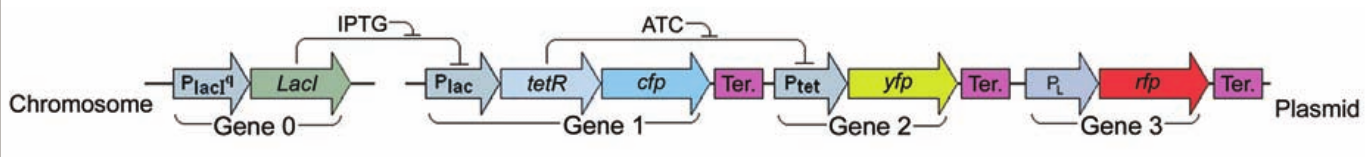
\includegraphics[width=15cm]{lan-circuit}
  \caption[Circuit used for the Langevin model]{\label{fig:lan-circuit} Circuit used in the Langevin model (from \cite{pedraza05}).}
\end{figure}

A similar effect happens on gene $2$, the tetracycline promoter P$_\text{tet}$, which regulated the expression of the yellow fluorescent protein \textit{yfp}. It is repressed by \textit{tetR} and the repressing effect of \textit{tetR} is also inhibited by ATC.

Therefore, both IPTG and ATC are environmental signals that are used to regulate the coupling between the different genes of the cascade. Notice that for instance, at higher quantities of IPTG, expression of gene $1$ is low since the repression over it is reduced. This also causes that without ATC, the expression of gene $2$ is high. 

The fluorescent proteins are used to quantify experimentally via fluorescence microscopy the expressions of each gene, which will be proportional to the intensity of the flourescence on each color. \textit{tetR} and \textit{cfp} are transcribed bicistronically in order to be able to quantify \textit{tetR} levels. We will assume that protein degradation is caused only by cell division (i.e. there is no active degradation). That allow us to use the same degradation constant for all proteins, and in particular, to assume that the behavior of \textit{cfp} reproduces exactly the behavior of \textit{tetR}. 

We will label the concentrations of \textit{LacI}, \textit{tetR} (and \textit{cfp}), \textit{yfp} and \textit{rfp} as $x_0$, $x_1$, $x_2$, and $x_3$, respectively.

\section{Mathematical derivations}

The differential equation for the mRNA will not be considered, we will write the equation for the proteins and include the effect of mRNA in the rate of creation $k$. The results of the previous chapter for the noise in proteins caused by mRNA will also be considered. The deterministic equation for the concentration of proteins of gene $0$ is 

\begin{equation}
\label{eq:detgene0}
\dot{x_0}(t) = k - \gamma x_0(t).
\end{equation}

Where now $k$ represents the average number of proteins created per unit time\footnote{For a better understanding of this point. If we assume $\gamma_p\ll\gamma_r$, we can treat the mRNA in steady state, hence eq. \eqref{eq:mas-simple_det_2} becomes eq. \eqref{eq:detgene0} with $k \coloneqq k_p\langle n_1\rangle_s =  \frac{k_pk_r}{\gamma_r} = k_rb$.}.

We will use the Langevin approach following the same procedures that were explained on the previous section. Here we add two noise terms to the deterministic equations representing the intrinsic noise $\mu_0(t)$ and the global noise $\xi_0(t)$. Hence, the equation for the stochastic process $x_0(t)$ is

\begin{equation}
\label{eq:gene0}
\dot{x_0}(t) = k - \gamma x_0(t) + \mu_0(t) + \xi_0(t).
\end{equation}

The noise terms have zero average, i.e.

\begin{equation*}
\langle\mu_0\rangle(t) = \langle\xi_0\rangle(t) = 0
\end{equation*}

and assuming white noise statistics for both sources, the autocorrelation functions are

\begin{align}
\langle\mu_0(t)\mu_0(t+\tau)\rangle&=q^2_{0,\text{int}}\delta(\tau)=2\gamma(b_0+1)\bar{x}_0\delta(\tau),\label{eq:corin0}\\
\langle\xi_0(t)\xi_0(t+\tau)\rangle&=q^2_{0,G}\delta(\tau)=2\gamma\eta_G^2\bar{x}_0^2\delta(\tau). \label{eq:corex0}
\end{align}

where $\eta_G$ is the strenght of the global noise, a parameter that is measured experimentally, and $b_0$ is the average number of protein produced per mRNA. In this section the bar denotes steady state average. Also, since both sources of noise are uncorrelated

\begin{equation}
\label{eq:corinex0}
\langle\mu_0(t)\xi_0(t+\tau)\rangle = 0.
\end{equation}

\todo[inline]{Understand and explain more the constants and the assumption of white noise}

We will derive the constant term in eq. \eqref{eq:corin0}. Notice that we can not use eq. \eqref{eq:lan-q_form} to find the factor $q$ in the correlations since with the assumptions made in eq. \eqref{eq:detgene0}, protein creation is not a one step Poisson process. From the results of section \label{sec:lan-single} we obtain comparing with eq. \eqref{eq:lan-qrel1}

\begin{equation*}
  \sigma^2(x_0) = \frac{q_{0,\text{int}}^2}{2\gamma}
\end{equation*}

and from eq. \eqref{eq:lan-simple_varp} we obtain

\begin{equation*}
  \bar{x}_0\left(\frac{b_0}{1+\gamma_p/\gamma_r}+1\right) = \frac{q_\text{int}^2}{2\gamma}.
\end{equation*}

The bar denotes steady state average. Since proteins are much more stable than mRNA, we can take $\gamma_p\ll\gamma_r$. With this approximation we get

\begin{equation*}
  q_{0,\text{int}}^2 \approx 2\gamma\bar{x}_0(b_0+1).
\end{equation*}

In fact, since intrinsic fluctuations depends only on the gene in question, the factor $q$ has the same form for all genes, i.e.

\begin{equation*}
  q_{i,\text{int}}^2 \approx 2\gamma\bar{x}_i(b_i+1),\quad i = 0,1,2,3.
\end{equation*}

In terms of $\delta x_0 \coloneqq x_0 - \bar{x}_0$, eq. \eqref{eq:gene0} becomes

\begin{equation}
\label{eq:dgene0}
\dot{\delta x_0}(t) = -\gamma \delta x_0(t) + \mu_0(t) + \xi_0(t).
\end{equation}

We will Fourier transform the equation, find its square norm and use the Wiener-Khinchin theorem (eq. \eqref{eq:con-wkth}) to find the autocorrelations in terms of the power spectrum and to write the power spectrum of $\mu(t)$ and $\xi(t)$ in terms of their autocorrelations.

OJO

Fourier transforming and recalling that $[\mathscr{F}(\frac{\mathrm{d}x(t)}{\mathrm{d}t})](\omega) = i\omega \mathscr{F}(x(t))(\omega)$ for a function of time $x(t)$, we obtain after solving for $\hat{\delta x_0}$

\begin{equation}
\label{eq:fgene0}
\hat{\delta x_0}(\omega) = \frac{\hat{\mu_0}+\hat{\xi_0}}{\gamma + i\omega}.
\end{equation}

Taking the square norm and averaging we get

\begin{equation}
\left\langle |\hat{\delta x_0}|^2 \right\rangle = \frac{\left\langle|\hat{\mu_0}|^2\right\rangle + \left\langle\hat{\mu_0}^*\hat{\xi_0}\right\rangle+\left\langle\hat{\mu_0}\hat{\xi_0}^*\right\rangle+\left\langle|\hat{\xi_0}|^2\right\rangle}{\gamma^2 + \omega^2},
\end{equation}

Using the Wiener-Khinchin theorem and eqs. \eqref{eq:corin0} - \eqref{eq:corinex0}

\begin{equation}
  \label{eq:pgene0}
  \begin{split}
    \left\langle |\hat{\delta x_0}|^2 \right\rangle &= \frac{\left(2\gamma(b_0+1)\bar{x_0}+ 2\gamma\eta_G^2\bar{x_0}^2\right)\mathscr{F}(\delta(t))}{\gamma^2+\omega^2}\\
    &=\frac{2\gamma\bar{x_0}^2\left(\nicefrac{(b_0+1)}{\bar{x_0}}+ \eta_G^2\right)}{\gamma^2+\omega^2},
  \end{split}
\end{equation}

where the cross terms are zero by eq. \eqref{eq:corinex0}. Applying the inverse Fourier transform at $t=0$ we get

\begin{equation*}
\langle \delta x_0^2 \rangle = 2\gamma\bar{x_0}^2\left(\nicefrac{(b_0+1)}{\bar{x_0}}+ \eta_G^2\right)\frac{1}{2\pi}\int_{-\infty}^{\infty}\frac{d\omega}{\omega^2+\gamma^2}
\end{equation*}

The integral can be easily solved by residues resulting in $\pi/\gamma$, therefore

\begin{equation*}
\langle \delta x_0^2 \rangle = \bar{x_0}^2\left(\frac{(b_0+1)}{\bar{x_0}}+ \eta_G^2\right)
\end{equation*}

And dividing by $\bar{x_0}^2$, we obtain the squared coefficient of variation

\begin{equation}
  \label{eq:etagene0}
  \boxed{\eta_0^2 = \frac{(b_0+1)}{\bar{x_0}}+ \eta_G^2 = \eta_{0,\text{int}}^2+\eta_G^2},
\end{equation}

where $\eta_{i,\text{int}}^2\coloneqq\frac{(b_i+1)}{\bar{x_i}}$ for $i=0,1,2,3$.

Therefore the total squared noise for gene $0$ is composed of the contributions from both the intrinsic and the global noise.

Now we will make the calculation for gene $1$, which follows the equation

\begin{equation}
\label{eq:gene1}
\dot{x_1}(t) = k_1(x_{0A})-\gamma x_1+\mu_1+\xi_1
\end{equation}

The creation rate $k_1$ is a Hill equation for repression where the repressor is $x_{0A}$, the amount of $x_0$ that is unbound to IPTG. The statistics for the noise terms are analogous to eqs. \eqref{eq:corin0} - \eqref{eq:corinex0}. We also need to know in this case the correlations between the noise terms corresponding to gene $0$ and the ones corresponding to gene $1$. As we have said, extrinsic sources of noise are uncorrelated

\begin{equation}
\label{eq:corcross01}
\langle\mu_0(t)\mu_1(t+\tau)\rangle = \langle\mu_0(t)\xi_1(t+\tau)\rangle = \langle\mu_1(t)\xi_0(t+\tau)\rangle = 0,
\end{equation}

but the extrinsic parts of the noise of genes $0$ and $1$ are correlated. In analogy with eq. \eqref{eq:corex0} we get

\begin{equation}
  \langle\xi_0(t)\xi_1(t+\tau)\rangle = 2\gamma\eta_G^2\bar{x_0}\bar{x_1}\delta(\tau).
\end{equation}

\todo[inline]{Also, understand and explain the q term here}

We proceed in a similar way to gene $0$. Defining $\delta x_1(t) \coloneqq x_1(t) - \bar{x_1}$, writing eq. \eqref{eq:gene1} in terms of $\delta x_1$, $\delta x_{0A}$, and making a Taylor expansion of $k_1$ to first order in $x_{0A}$ about $\bar{x}_{0A}$ we obtain.

\begin{equation}
\dot{\delta x_1} = k_1(\bar{x_{0A}}) + \left.\frac{dk_1(x_{0A})}{dx_{0A}}\right|_{\bar{x_{0A}}}\delta x_{0A} - \gamma(\delta x_1 + \bar{x_1}) + \mu_1 + \xi_1,
\end{equation}

but from eq. \eqref{eq:gene1}, $\bar{x_1} = \nicefrac{k_1(\bar{x_{0A}})}{\gamma}$, therefore

\begin{equation}
  \label{eq:dgene1}
  \dot{\delta{x_1}(t)}=c_1\delta x_{0A}-\gamma\delta x_1 + \mu_1 \xi_1,
\end{equation}

where $c_1 \coloneqq \left.\nicefrac{dk_1(x_{0A})}{dx_{0A}}\right|_{\bar{x_{0A}}}$ Fourier transforming and solving for $\hat{\delta x_1}$ we get

\begin{equation*}
  \hat{\delta x_1}=\frac{c_1\hat{\delta x_{0A}}+\hat{\mu_1}+\hat{\xi_1}}{\gamma + i\omega}.
\end{equation*}

Taking the square norm and averaging

\begin{equation*}
  \label{eq:pgene1}
  \begin{split}
    \left\langle|\hat{\delta x_1}|^2\right\rangle &= \frac{1}{\omega^2+\gamma^2}\left(c_1\hat{\delta x_{0A}} + \hat{\mu_1} + \hat{\xi_1}\right)\left(c_1\hat{\delta x_{0A}}^* + \hat{\mu_1}^* + \hat{\xi_1}^*\right)\\
    &=\frac{1}{\omega^2+\gamma^2}\left(c_1^2 \left\langle|\hat{\delta x_{0A}}|^2\right\rangle + c_1\left(\langle\hat{\delta x_{0A}}\hat{\xi_1}^*\rangle+\langle\hat{\delta x_{0A}}^*\hat{\xi_1}\rangle\right) +  \left\langle|\hat{\mu_1}|^2\right\rangle +  \left\langle|\hat{\xi_1}|^2\right\rangle\right)
  \end{split}
\end{equation*}

Using the Wiener-Khinchin theorem and the equations for the correlations we get

\begin{align*}
  \left\langle|\hat{\mu_1}|^2\right\rangle &= 2\gamma(b_1+1)\bar{x_1},\\
  \left\langle|\hat{\xi_1}|^2\right\rangle &= 2\gamma\eta_G^2\bar{x_1}^2,
\end{align*}

since the Fourier transform of the Dirac delta is $1$. Usually the binding and unbinding of inducers such as $IPTG$ occurs at timescales that are much smaller than the timescales of transcription and translation. Therefore, time averaging makes those fluctuations negligible. With this in mind, we will assume that the noise in $x_{0A}$ are the same as the noise in $x_0$. Then from eqs. \eqref{eq:fgene0} and \eqref{eq:pgene0} we get

\begin{align*}
\left\langle|\hat{\delta x_{0A}}|^2\right\rangle &= \frac{2\gamma\bar{x_0}^2\left(\nicefrac{(b_0+1)}{\bar{x_0}}+ \eta_G^2\right)}{\gamma^2+\omega^2},\\
\langle\hat{\delta x_{0A}}\hat{\xi_1}^*\rangle &= \frac{1}{\gamma+i\omega}\left(\langle\hat{\mu_0}\hat{\xi_1}^*\rangle + \langle\hat{\xi_0}\hat{\xi_1}^*\rangle \right) = \frac{\langle\hat{\xi_0}\hat{\xi_1}^*\rangle}{\gamma+i\omega}\\
\langle\hat{\delta x_{0A}}^*\hat{\xi_1}\rangle &= \frac{1}{\gamma-i\omega}\left(\langle\hat{\mu_0}^*\hat{\xi_1}\rangle + \langle\hat{\xi_0}^*\hat{\xi_1}^*\rangle \right) = \frac{\langle\hat{\xi_0}^*\hat{\xi_1}\rangle}{\gamma-i\omega}
\end{align*}

Where the last step in the last two equations comes from the Wiener-Khinchin theorem and eq. \eqref{eq:corcross01}. Replacing the previous equations in eq. \eqref{eq:pgene1} and taking the inverse transform we get for the variance

\begin{equation*}
  \begin{split}
    \langle \delta x_1^2\rangle &= 2\gamma\bar{x_0}^2c_1^2\left(\nicefrac{(b_0+1)}{\bar{x_0}}+ \eta_G^2\right)\frac{1}{2\pi}\int_{-\infty}^{\infty}\frac{d\omega}{(\omega^2+\gamma^2)^2}\\
    &+2\gamma\eta_G^2\bar{x_0}\bar{x_1}c_1\frac{1}{2\pi}\left(\int_{-\infty}^{\infty}\frac{d\omega}{(\gamma + i\omega)(\omega^2+\gamma^2)} + \int_{-\infty}^{\infty}\frac{d\omega}{(\gamma - i\omega)(\omega^2+\gamma^2)}\right)\\
    &+2\gamma\bar{x_1}^2 \left(\nicefrac{(b_1+1)}{\bar{x_1}}+\eta_G^2\right)\frac{1}{2\pi}\int_{-\infty}^{\infty}\frac{d\omega}{\omega^2+\gamma^2}.
  \end{split}
\end{equation*} 

Solving the integrals in the complex plane and rearranging

\begin{equation*}
  \langle \delta x_1^2\rangle = \frac{c_1^2\bar{x_0}^2}{2\gamma^2}\left(\nicefrac{(b_0+1)}{\bar{x_0}}+ \eta_G^2\right) + \frac{c_1\eta_G^2\bar{x_0}\bar{x_1}}{\gamma} + \bar{x_1}^2\left(\nicefrac{(b_1+1)}{\bar{x_1}}+\eta_G^2\right).
\end{equation*}

Dividing by $\bar{x}_1^2$ yields

\begin{equation}
  \label{eq:lan-eta1_alm}
  \eta_1^2 = \frac{1}{2}\frac{c_1^2\bar{x_0}^2}{\gamma^2\bar{x}_1^2}\left(\frac{(b_0+1)}{\bar{x_0}}+ \eta_G^2\right) + \frac{c_1\bar{x_0}}{\gamma \bar{x}_1}\eta_G^2 + \frac{(b_1+1)}{\bar{x_1}}+\eta_G^2.
\end{equation}


Recall the definition of the logarithmic gain from eq. \eqref{eq:fdt-def_H}

\begin{equation*}
  H_{10} = \frac{\partial \ln (\langle J_1^-\rangle/\langle J_1^+\rangle)}{\partial \ln \langle x_0\rangle}.
\end{equation*}

From eq. \eqref{eq:gene1}, we have $\langle J_1^+\rangle = k_1(\bar{x}_{0A})$ and $\langle J_i^-\rangle = \gamma \bar{x}_1$. Then,

\todo[inline]{Aqui que con el promedio si la func es nonlinear}

\begin{equation*}
  H_{10} = \frac{\partial \ln\left(\frac{\gamma\bar{x}_1}{k1(\bar{x}_{0A})}\right)}{\partial \ln  \bar{x}_0} = -\frac{\frac{\gamma \bar{x}_1}{k_1(\bar{x}_{0A})}\partial\left(\frac{k_1(\bar{x}_{0A})}{\gamma \bar{x}_1}\right)}{\frac{\partial \bar{x}_{0A}}{\bar{x}_{0A}}} = -\frac{\bar{x}_{0A}}{k_1(\bar{x}_{0A})}\frac{\mathrm{d} k_1(\bar{x}_{0A})}{\mathrm{d} \bar{x}_{0A}} = -\frac{c_1 \bar{x}_{0A}}{\gamma\bar{x}_1}.
\end{equation*}

Since gene $2$ has the same dependence on the number of active proteins of gene $1$ (not bound to ATC), we have in general

\begin{equation}
  \label{lan-Hexp}
  H_{ij} = \frac{c_i \bar{x}_{jA}}{\gamma\bar{x}_i} = \frac{\bar{x}_{jA}}{\gamma\bar{x}_i}\frac{\mathrm{d}k_i(\bar{x}_{jA})}{\mathrm{d} \bar{x}_{jA}},\quad\text{for}\quad (i,j) = \{(1,0),(2,1)\}.
\end{equation}

Replacing this in eq. \eqref{eq:lan-eta1_alm} we obtain

\begin{equation}
  \label{eq:etagene1}
  \begin{split}
    \eta_1^2 &= \eta_{1\text{int}}^2 + \frac{1}{2}H_{10}^2\eta_0^2+\eta_G^2\left(1-H_{10}\right)\\
    &= \eta_{1\text{int}}^2+\frac{1}{2}H_{10}^2\eta_{0\text{int}}^2+\eta_G^2\left(1+ \frac{1}{2}H_{10}^2-H_{10}\right),
  \end{split}
\end{equation}

where $\eta_{1\text{int}}^2 = \frac{(b_1+1)}{\bar{x_1}}$ and $\eta_0^2$ is given by eq. \ref{eq:etagene0}.

This corroborates what was said at the end of chapter \ref{ch:fdt}. The total noise in gene one is given by the intrinsic part, the noise from gene $0$ that is propagated to gene $1$ (including both its intrinsic and global part) and the global noise that enters directly into gene $1$. The factor of $1/2$ represents the time averaging since we assumed equal degradation rates for both proteins.

For gene $2$ we proceed similarly, with analogous statistics for the noise terms, the resulting noise is

\begin{equation}
  \label{eq:etagene2}
  \begin{split}
    \eta_2^2 &= \eta_{2\text{int}}^2 +  \frac{1}{2}H_{21}^2\eta_{1\text{int}}^2+\frac{3}{8}H_{21}^2H_{10}^2\eta_{0\text{int}}^2\\
    &+\eta_G^2\left(1 + \frac{1}{2}H_{21} + \frac{3}{8}H_{21}^2H_{10}^2 - H_{21} -\frac{3}{4}H_{21}^2H_{10} + \frac{1}{2}H_{21}H_{10}\right),\\
    &= \eta_{2\text{int}}^2 + \frac{1}{2}H_{21}^2\eta_1^2+\frac{1}{8}H_{21}^2H_{10}^2\eta_0^2+\eta_G^2\left(1-H_{21}-\frac{1}{4}H_{21}^2H_{10}+\frac{1}{2}H_{21}H_{10}\right).
  \end{split}
\end{equation}

Which contains the intrinsic noise of gene $2$, the contribution from the total noise of gene $1$, the contribution from the total noise of gene $0$ that is transmitted first to gene $1$ and then to gene $2$ and the global noise that enters directly. Notice that the time average factor for a two step propagation of intrinsic noise is less than $1/2$, verifying the conclusions of the previous section.

Since gene $3$ has also a constitutive promoter, its noise is given by

\begin{equation}
  \label{eq:etagene3}
  \eta_3^2 = \eta_{3\text{int}}^2+\eta_G^2.
\end{equation}

This gene was used to measure the strenght of the global noise $\eta_G$ since it is not connected with other components and thus it does not receives propagated noise. The correlations can be found in a very similar way. They are given by

\begin{equation}
  \label{eq:lan-correl}
  \begin{split}
    C_{12}&=-\frac{1}{2}H_{21}\eta_{1\text{int}}^2 -\frac{3}{8}H_{21}H_{10}^2\eta_{0\text{int}}^2+\eta_G^2\left(1-\frac{1}{2}H_{21}-\frac{1}{2}H_{10}-\frac{3}{8}H_{21}H_{10}^2 + \frac{3}{4}H_{21}H_{10}\right),\\
    C_{13}&=\eta_G^2\left(1-\frac{1}{2}H_{10}\right),\\
    C_{23}&=\eta_G^2\left(1-\frac{1}{2}H_{21}+\frac{1}{4}H_{21}H_{10}\right).
  \end{split}
\end{equation}

From the results it is clear that the noise is strongly dependent on the details of the network and on how is the interaction between the different components of the genetic circuit. A detailed analysis of these results will be done in the next section.

\section{Explicit expressions for the logarithmic gain}

The repressions between the genes of the cascade are mathematically represented writing the rates of creation as Hill type functions. They are given by

\begin{equation}
  \label{eq:lan-hill_g}
  \begin{split}
    k_1(y_{0A}) &= \alpha_1 + \frac{\beta_1}{1+(\frac{y_{0A}}{K_{d1}})^{h_1}},\\
    k_2(y_{1A}) &= \alpha_2 + \frac{\beta_2}{1+(\frac{y_{1A}}{K_{d2}})^{h_2}}.
\end{split}
  \end{equation}

The fraction of $y_0$ (\textit{LacI}) and $y_1$ (\textit{tetR}) that are unbound to ATC is also modeled as a Hill function i.e. $y_{0A} = k_0(IPTG)y_0$ and $y_{1A} = k_a(ATC)y_1$ where

\begin{equation}
  \begin{split}
    k_0(IPTG) &= \alpha_0 + \frac{\beta_0}{1+(\frac{IPTG}{K_{d0}})^{h_0}},\\
    k_2(y_{1A}) &= \alpha_a + \frac{\beta_a}{1+(\frac{ATC}{K_{da}})^{h_a}}.
\end{split}
  \end{equation}

To find the logarithmic gains $H_{21}$ and $H_{10}$, we use eq. \eqref{lan-Hexp} and eq. \eqref{eq:lan-hill_g} to obtain after differentiating for $(i,j) = \{(1,0),(2,1)\}$

\begin{equation}
  \label{eq:lan-H_det}
  H_{ij} = \frac{\bar{x}_{jA}}{\gamma\bar{x}_i}\frac{\mathrm{d}}{\mathrm{d} \bar{x}_{jA}}\left( \alpha_i + \frac{\beta_i}{1+(\frac{\bar{x}_{jA}}{K_{di}})^{h_i}}\right) = \frac{h_i}{\beta_i k_i(\bar{x}_{jA})}\left(k_i(\bar{x}_{jA}) - \alpha_i\right) \left(\alpha_i+\beta_i-k_i(\bar{x}_{jA})\right).
\end{equation}

The values of the parameters that will be used in the following calculations and graphics can be found in github \footnote{The equations were solved and plotted using Wolfram Mathematica. The notebook, which also contains the values for the parameters can be found in \url{https://github.com/gutiloluis/61Monograph/blob/master/math/lan-analytic_solver.nb}. Most of the parameters were fitted experimentally by Pedraza and van Oudenaarden \cite{pedraza05}}. 

Replacing eqs. \eqref{eq:lan-hill_g} - \eqref{eq:lan-H_det} we obtain explicit expressions for the logarithmic gains that, given the values of the parameters can be replaced in the eqs. for the noises and correlations. Fig. \ref{fig:lan-Hs} shows the logarithmic gains as a function of [IPTG] when [ATC] = 0.

\begin{figure}[H]
  \centering
  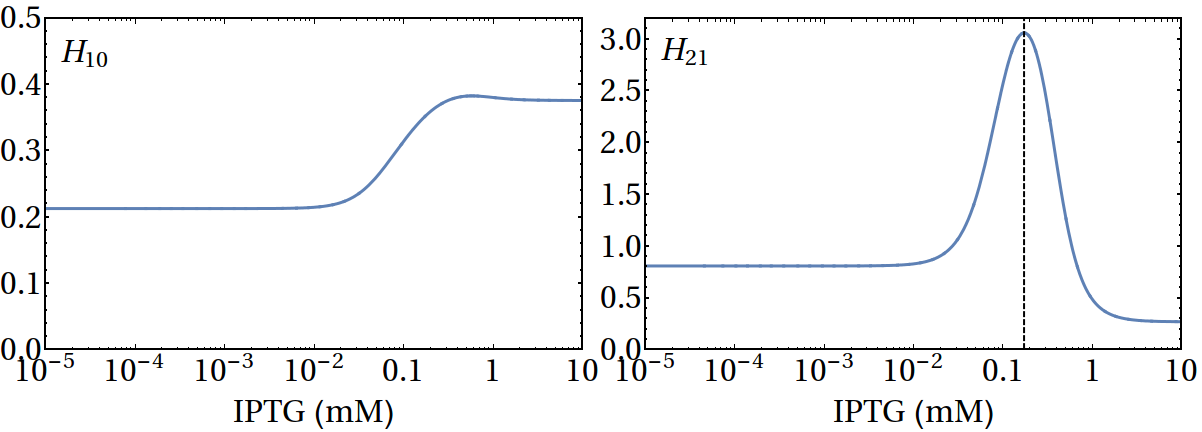
\includegraphics[width=15cm]{lan-Hs}
  \caption[Logarithmic gains for the genes of a cascade]{\label{fig:lan-Hs}. Plot of $H_{21}$ and $H_{10}$ as a function of [IPTG] given by eq. \eqref{eq:lan-H_det} . The vertical line marks the maximum of $H_{21}$.}
\end{figure}

The maximum value in $H_{21}$ represents the concentration of [IPTG] at which $y_2$ is more affected by changes in $y_1$. This corresponds to the point of the transfer function where the slope is greater. At this level of [IPTG] the noise transmitted from $y_1$ to $y_2$ is increased.

Figure \ref{fig:lan-noise_corr_full} shows the noises and correlations for certain set of values of the parameters as a function of the concentration of IPTG when there is no ATC.

\begin{figure}[H]
  \centering
  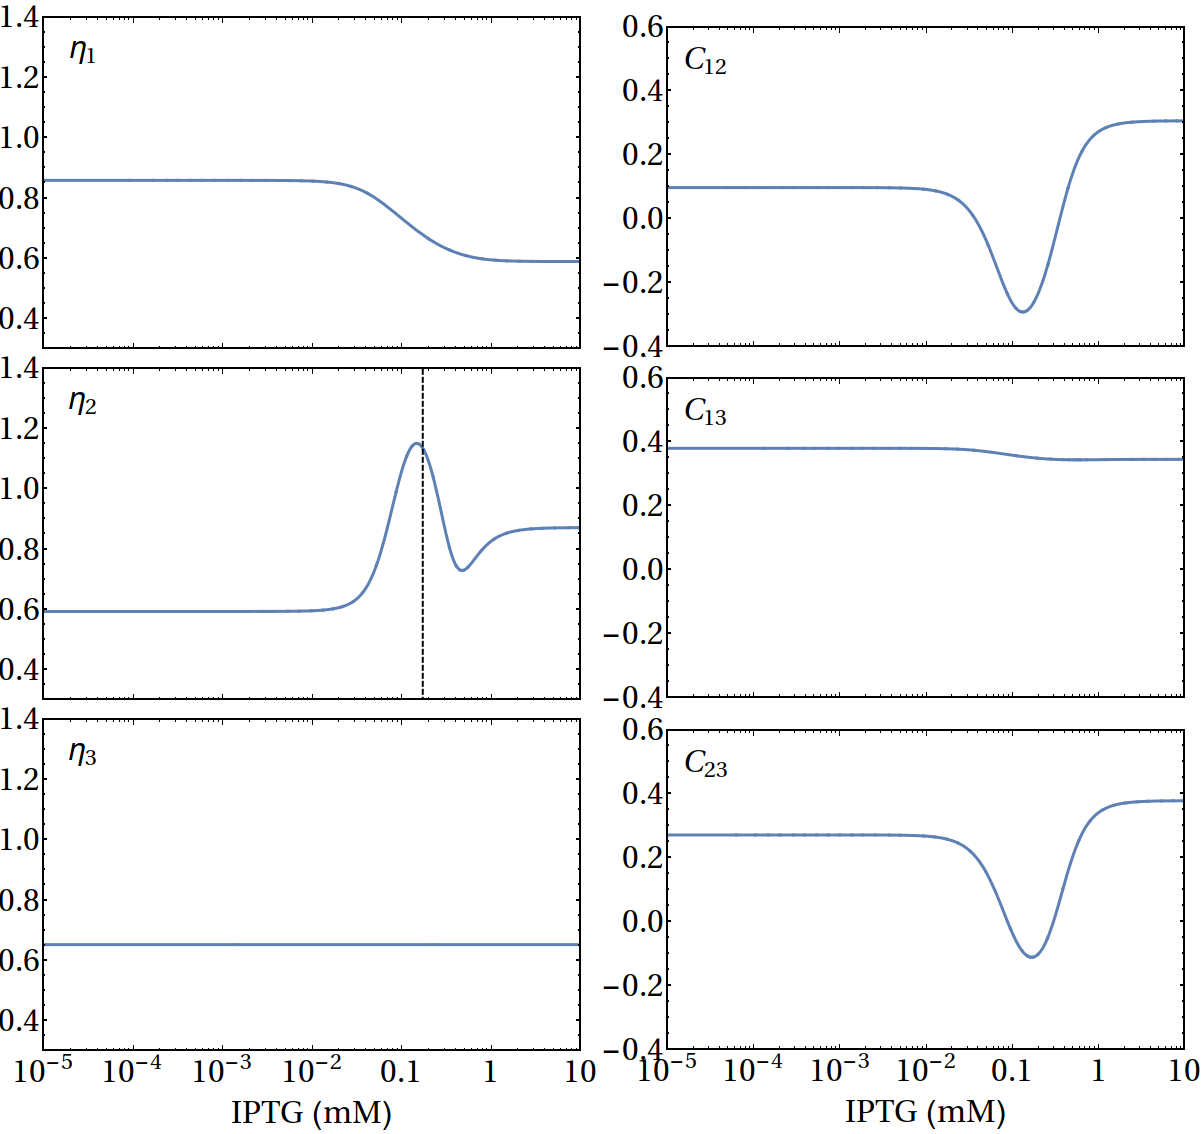
\includegraphics[width=15cm]{lan-noise_corr_full}
  \caption[Noises and correlation for the genes of a cascade]{\label{fig:lan-noise_corr_full}. Plot of noises (eqs. \eqref{eq:etagene3} and \eqref{eq:etagene3}) and correlations (\eqref{eq:lan-correl}) as a function of [IPTG] for genes $1$ to $3$ with [ATC]=0. The vertical line shows the IPTG concentration at which $H_{21}$ reaches its greater value.}
\end{figure}

The noise in $\eta_3$ is constant since it is not part of the cascade. Also, the noise in gene $1$ is reduced as IPTG is increased because . The noise in gene $2$ has its maximum almost at the point of greater logarithmic gain as we said earlier. This evidences the fact that the noise is strongly dependent on the propagation from interacting components. It does not match exactly as a consequence of the other sources of noise.

From eqs. \eqref{eq:etagene1} and \eqref{eq:etagene2} it can be seen that the intrinsic propagated noise always depends on the square of the logarithmic gain while the global propagated noise has terms that depend on its sign. This is a consequence of the correlation of the global noise among all the genes.

ANALYZE THE CORRELATION BETWEEN GENE 1 AND 3, AMAZING.

\begin{figure}[H]
  \centering
  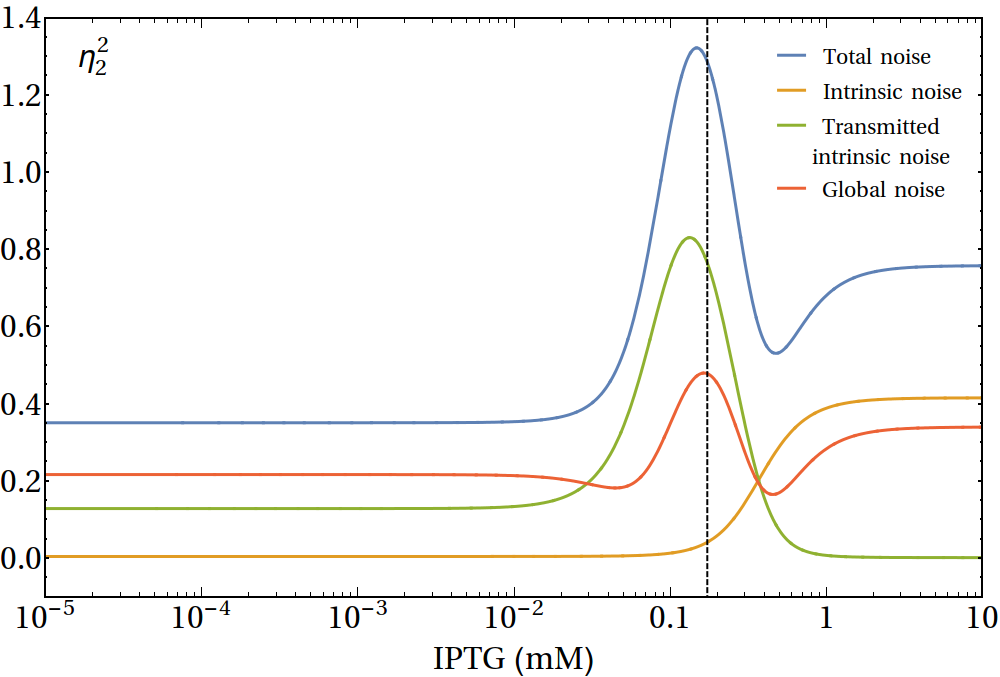
\includegraphics[width=15cm]{lan-eta2det}
  \caption[Components of the noise]{\label{fig:lan-eta2det}. Plot of each component of $\eta_2^2$ (eq. \eqref{eq:etagene2}) as a function of [IPTG] with [ATC]=0. The vertical line shows the IPTG concentration at which $H_{21}$ reaches its greater value.}
\end{figure}


\begin{figure}[H]
  \centering
  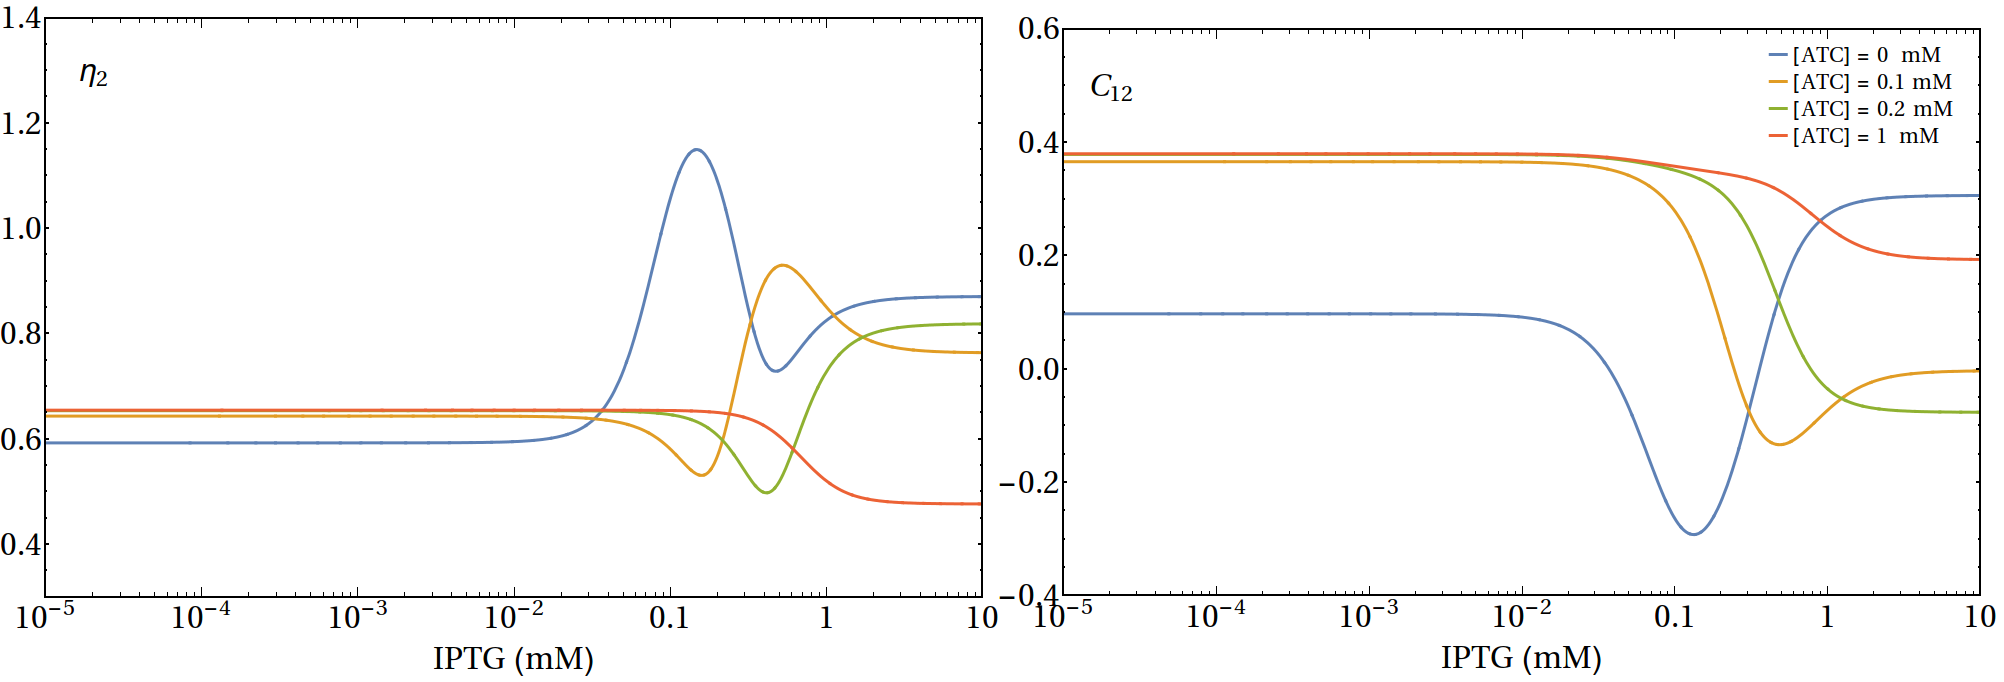
\includegraphics[width=15cm]{lan-eta2_corrATC}
  \caption[Noise in gene $2$ for varying ATC concentrations]{\label{fig:lan-eta2_corrATC}. Plots of $\eta_2$ (eq. \eqref{eq:etagene2}) and $C_{12}$ (eq. \eqref{eq:lan-correl}) as a function of [IPTG] for different ATC concentration shown in the legend.}
\end{figure}

As it can be noticed in eqs. \eqref{eq:etagene0}, \eqref{eq:etagene1} and \eqref{eq:etagene2}, the noise propagation follows the sequence of fig. \ref{fig:lan-noise_sources}. For each gene there is an independent intrinsic noise a correlated global noise, and both the transmitted global and intrinsic noise between the genes of the cascade whose strenght is determined by the logarithmic gain $H$.

\begin{figure}[H]
  \centering
  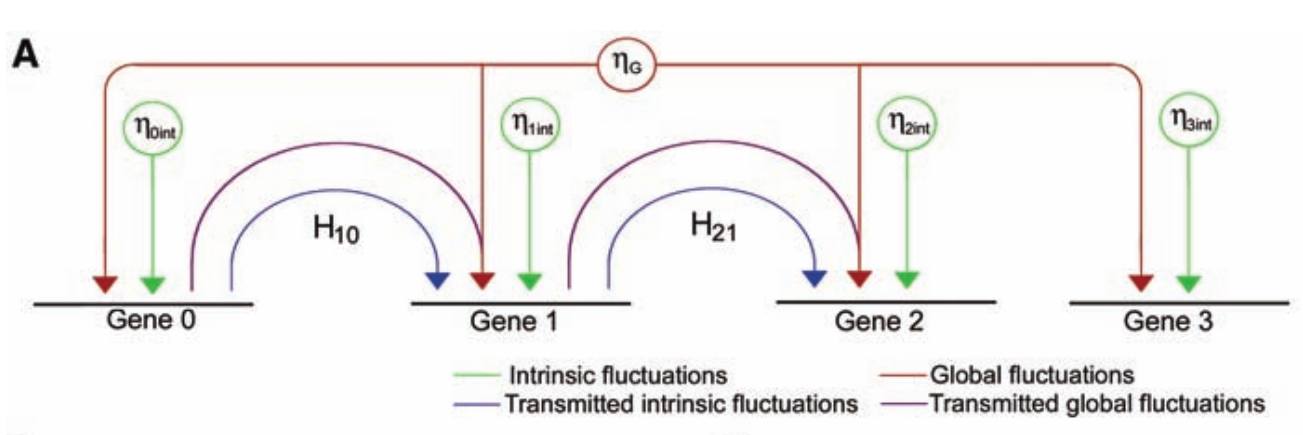
\includegraphics[width=15cm]{lan-noise_sources}
  \caption[Propagation of noise through a cascade]{\label{fig:lan-noise_sources} Different sources of noise and their propagation along the cascade of regulation (from \cite{pedraza05}).}
\end{figure}

\todo[inline]{TODO: Analyze the results physically (recall SysBio class), reproduce the graphics and analyze them}

This approach enables us to calculate the coefficient of variation for a cascade of regulation and separate the different sources of noise. Also, it enables to write the effect of the upstream genes in terms of the logarithmic gain, making it very intuitive. The results of the theoretical model were tested with experiments where the genes that are part of the cascade are transcribed bicistronicaly with fluorescent reporters. The fluctuations in the intensity of the reporters was used to measure the noise in the population of cells.
